% Este archivo es parte de la memoria del proyecto fin de carrera
% de Manuel López Urbina. Protegida bajo la licencia GFDL.
% Para más información, la licencia completa viene incluida en el
% fichero fdl-1.3.tex

% Copyright (C) 2018 Manuel López Urbina

\newpage

\chapter{Introducción}
\label{chap:introducción}

La robótica es una rama de la ingeniería, la cual se ocupa del diseño, construcción, operación y uso de robots\footnote{Robot: Máquina automática programable capaz de 
realizar determinadas operaciones de manera autónoma y sustituir a los seres humanos en algunas tareas, en especial las pesadas, repetitivas o peligrosas; puede estar dotada de sensores, 
que le permiten adaptarse a nuevas situaciones.}, así como sistemas informáticos para su control, retroalimentación sensorial y procesamiento de información. Entre las diversas
disciplinas aplicadas a la robótica podemos encontrar: la mecánica, la electrónica, la informática, la inteligencia artificial, la ingeniería de control y la física, entre otras muchas. De lo cual podemos considerar 
la robótica como una ciencia multidisciplinar.\\

Un robot es, por tanto, una máquina capaz de interactuar con su entorno. Si es móvil, a menos que se mueva en un espacio absolutamente acotado y preparado para él, deberá ser
capaz de adaptar sus movimientos y sus acciones de interacción en base a las características físicas de los ambientes con los que se encuentre y los objetos que hay en ellos.\\

Para lograr esta capacidad de adaptación, lo primero que necesitan los robots es tener conocimiento del entorno, resultando ésto absolutamente imprescindible. Para conocer el
entorno los seres vivos recibimos la información mediante los sentidos. Los robots, en infinidad de ocasiones buscando su inspiración en la naturaleza, deben disponer de sistemas que
les permitan saber dónde se encuentran, cómo es el lugar en el que están, a qué condiciones físicas se enfrentan, dónde están los objetos con los que deben interactuar,
sus parámetros físicos, etc.\\

Para esto se utilizan diversos tipos de sensores (o captadores), con un rango de complejidad y sofisticación que varía desde algunos bastante simples a otros con altos niveles de 
sofisticación de hardware y más aún de complejidad de programación.\\

Un sensor\footnote{En el capítulo de conceptos básicos, \ref{sec:sensor-definicion} puede acceder a información más detallada sobre los sensores, descripción, características, etc}
consta de algún elemento sensible a una magnitud física, como por ejemplo la intensidad o color de la luz, temperatura, presión, magnetismo, humedad, y debe ser capaz,
por su propias características, o por medio de dispositivos intermedios, de transformar esa magnitud física en un cambio eléctrico que se pueda alimentar en un circuito para
que la utilice directamente, o bien, pasando por una etapa previa que la condicione (amplificando, filtrando, etc.). Todo ello para que una vez procesada la señal por el robot
 éste actúe en consecuencia al parámetro recibido.\\

En la actualidad, estos sensores se encuentran presentes en robots de todo tipo. Éstos robots son muy utilizados en plantas de fabricación, montaje y embalaje, en transporte, en exploraciones en la Tierra y en el espacio, cirugía, armamento, investigación en laboratorios y 
en la producción en masa de bienes industriales o de consumo. También resultan de gran utilidad en la resolución de tareas peligrosas, existiendo multitud de aplicaciones como, 
limpieza de residuos tóxicos, minería, búsqueda, rescate de personas y localización de minas terrestres o accidentes nucleares.\\

Por tanto, centrándonos en el área de resolución de tareas peligrosas para las personas, un robot debe cumplir una serie de requerimientos para que cumpla adecuadamente con una serie 
de cometidos:\\

\begin{itemize}
 \item La movilidad y destreza para maniobrar en zonas con multitud de obstáculos típicos de las zonas de desastre.
 \item Capacidad de manipular y utilizar un surtido diverso de herramientas diseñadas para los seres humanos.
 \item Capacidad para ser manejado por los seres humanos que hayan tenido poca o ninguna formación robótica.
 \item Autonomía parcial en el nivel de tarea de toma de decisiones sobre la base de los comandos del operador y entradas de los sensores.
\end{itemize}

De todo lo anterior se extrae, por tanto, la necesidad de elaborar un sistema robótico operado por una persona y que permita el análisis del entorno, junto con la posibilidad de controlarlo mediante una 
aplicación software y una conexión a internet. O lo que es lo mismo, un sistema de \texbf{telemetría}\footnote{En el capítulo de conceptos básicos puede acceder a un apartado específico destinado a la telemetría \ref{def:telemetria}}.\\

La telemetría es una tecnología que está en pleno auge al permitir recibir información de un entorno sin necesidad de estar en él presente. 
La información que se desee medir para posteriormente transmitirla puede ser muy variada, según la situación. Desde el punto de vista de la comunicación, la información que se 
transmite es irrelevante, por lo que una vez establecida la forma en la que se envían y se reciben los datos, podremos añadir, reemplazar o modificar los sensores para adaptar el
proyecto tipo desarrollado a un entorno concreto o diferente al inicialmente pensado.\\

Así que dadas las motivaciones existentes y, junto que la programación web y la robótica son temas que causan en mi un especial interés, hicieron que me lanzara a la elaboración de este
proyecto que unifica ambos campos anteriormente citados.\\

Así surgió \emph{SensorRS, Multi-sensor Robot Sysmtem}.\\

\begin{figure}[H]
  \begin{center}
    
\includegraphics[scale=0.8]{imagenes/logotipo_sensor_rs.png}
  \end{center}
  \label{fig:logo}
 \caption{Logo SensorRS \protect\footnotemark.}
\end{figure}

\footnotetext{Logotipo de \emph{SensorRS}, Multi-sensor Robot Sysmtem.}

\emph{SensorRS, Multi-sensor Robot System} (nombre del sistema resultante) será una combinación de un elemento software (aplicación web RobotUI) y hardware (SensorRC, Multisensor
Robot System) surgido como un sistema para sacar el máximo aprovechamiento de la aplicación RobotUI para la que se eleborará un dispositivo robótico de propósito general cuya finalidad es
análisis y exploración del entorno gracias a los sensores incorporados.\\

SensorRS se compone de un vehículo controlado vía WiFi el cual responde a una serie de señales, \emph{comandos}\footnote{ Comando: instrucción u orden que el usuario proporciona a un sistema informático, 
desde la línea de comandos (como una shell) o desde una llamada de programación.}, a los que responde realizando determinadas acciones. Por otra parte también dispone de una cámara para la captura de imágenes.\\

La interfaz de control generada en la aplicación web RobotUI\footnote{ Aplicación anteriormente desarrollada por Manuel López Urbina para el control de dispositivos robóticos de propósito general. Acceso al 
código fuente: \url{https://github.com/lopi87/SAILS-RobotUI}}, se configurará de tal manera que permita el control del vehículo desarrollado en el presente proyecto. 
Esta aplicación permite dar de alta dispositivos robóticos para su control y retransmisión de su funcionamento en vivo con otros usuarios.\\


\begin{figure}[H]
    \centering
    \begin{subfigure}[b]{0.3\textwidth}
        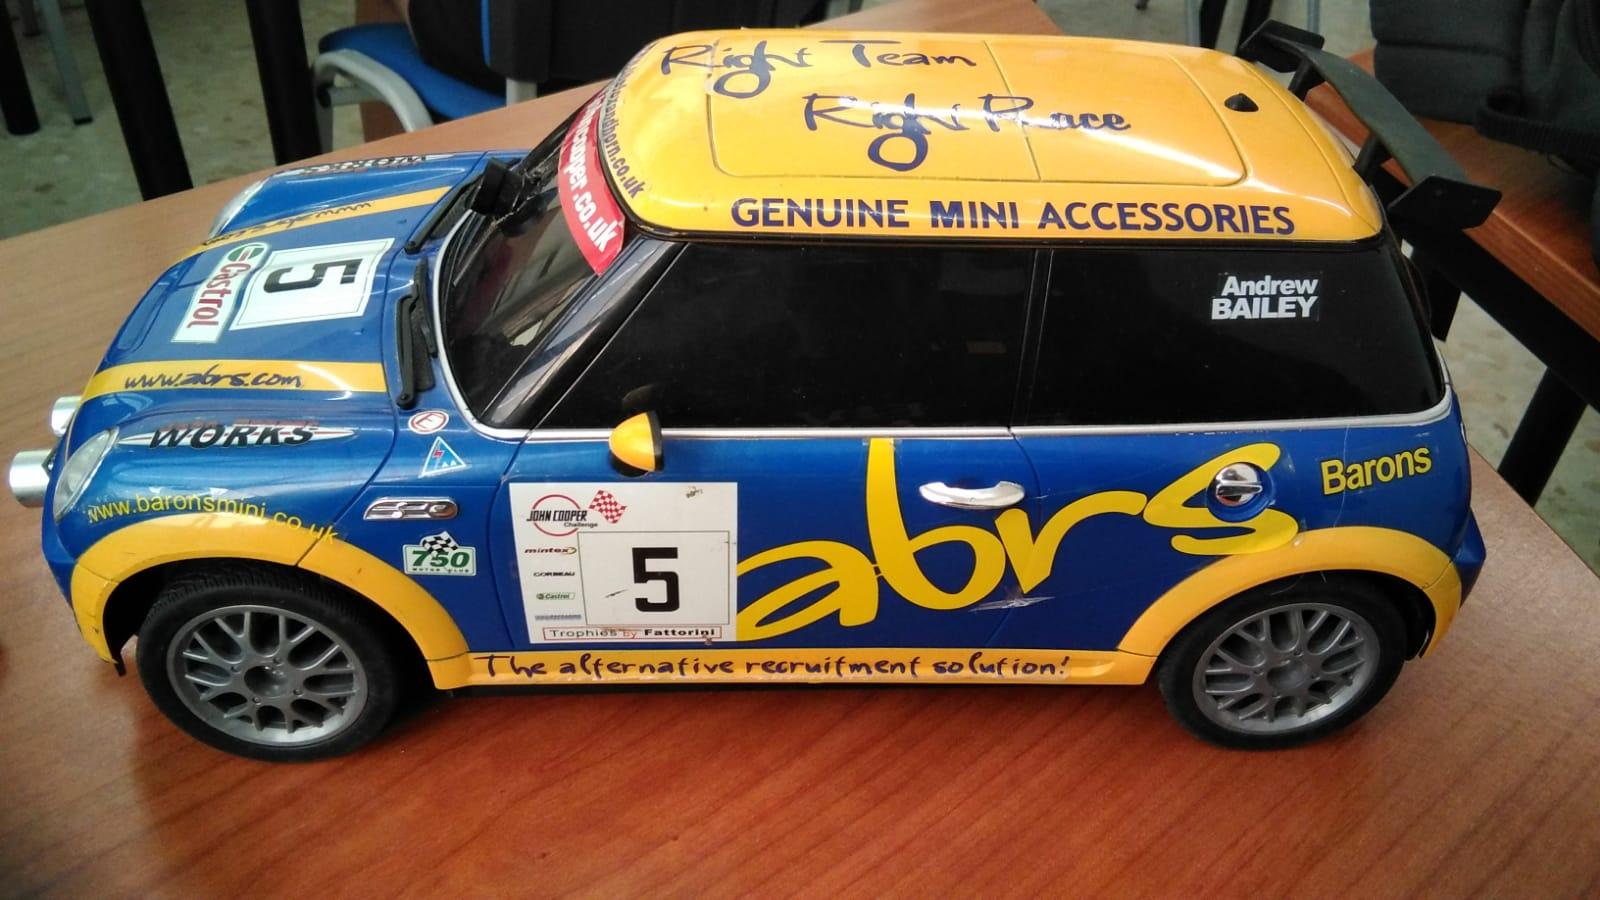
\includegraphics[width=\textwidth]{imagenes/robot/vehiculo_lateral.jpeg}
        \caption{Vista lateral}
        \label{fig:gull}
    \end{subfigure}
    \begin{subfigure}[b]{0.3\textwidth}
        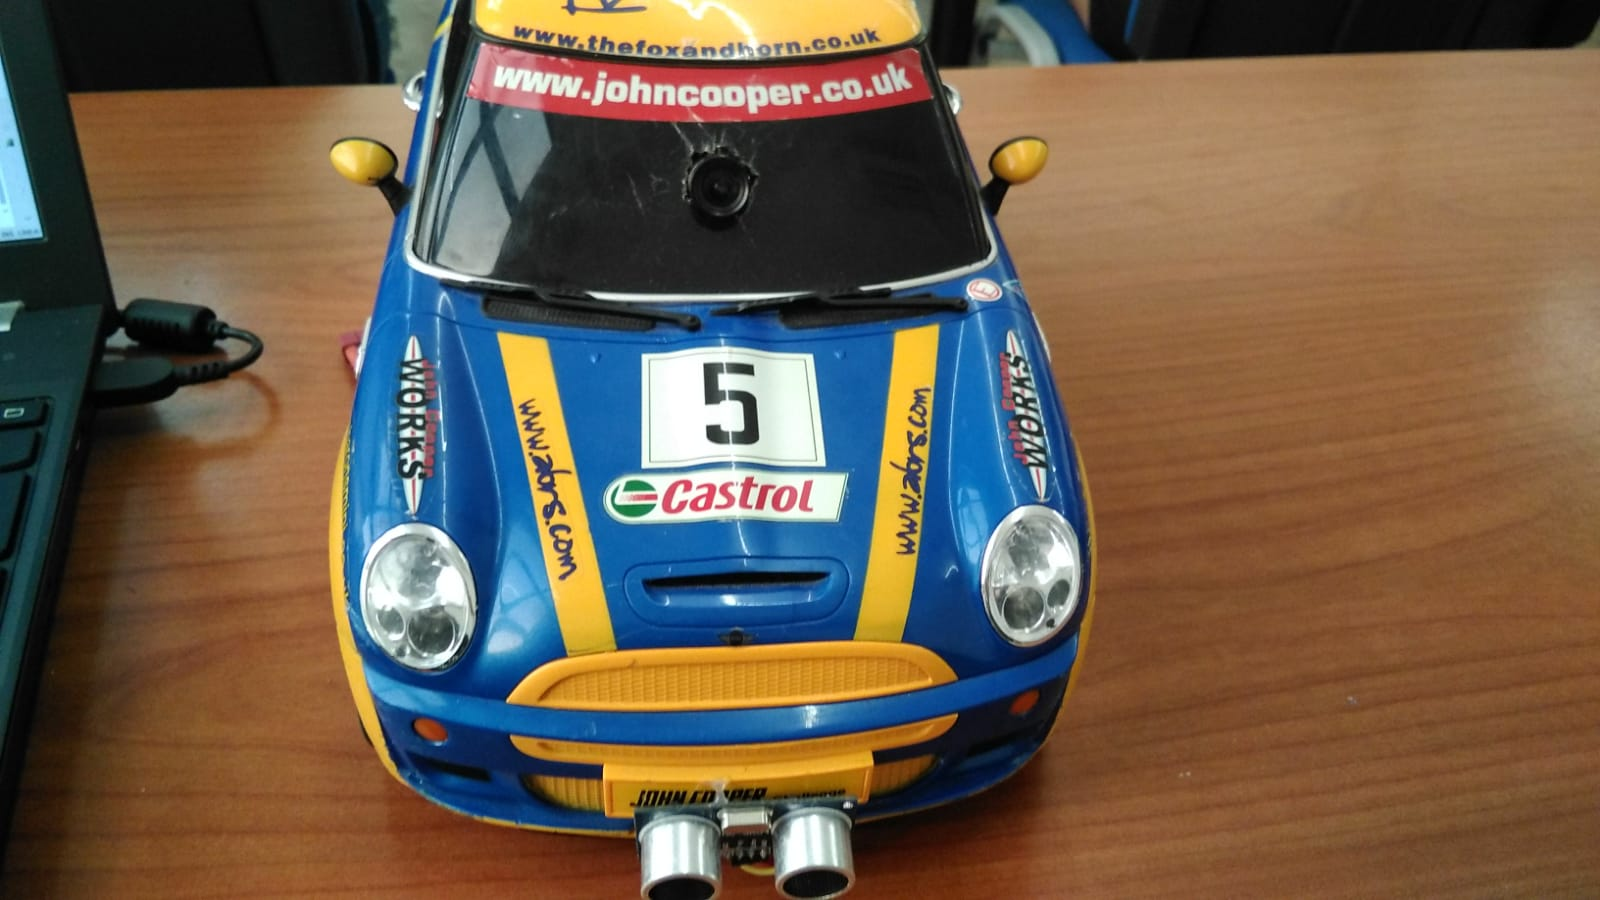
\includegraphics[width=\textwidth]{imagenes/robot/vehiculo_frontal.jpeg}
        \caption{Vista frontal}
        \label{fig:tiger}
    \end{subfigure}
    \begin{subfigure}[b]{0.3\textwidth}
        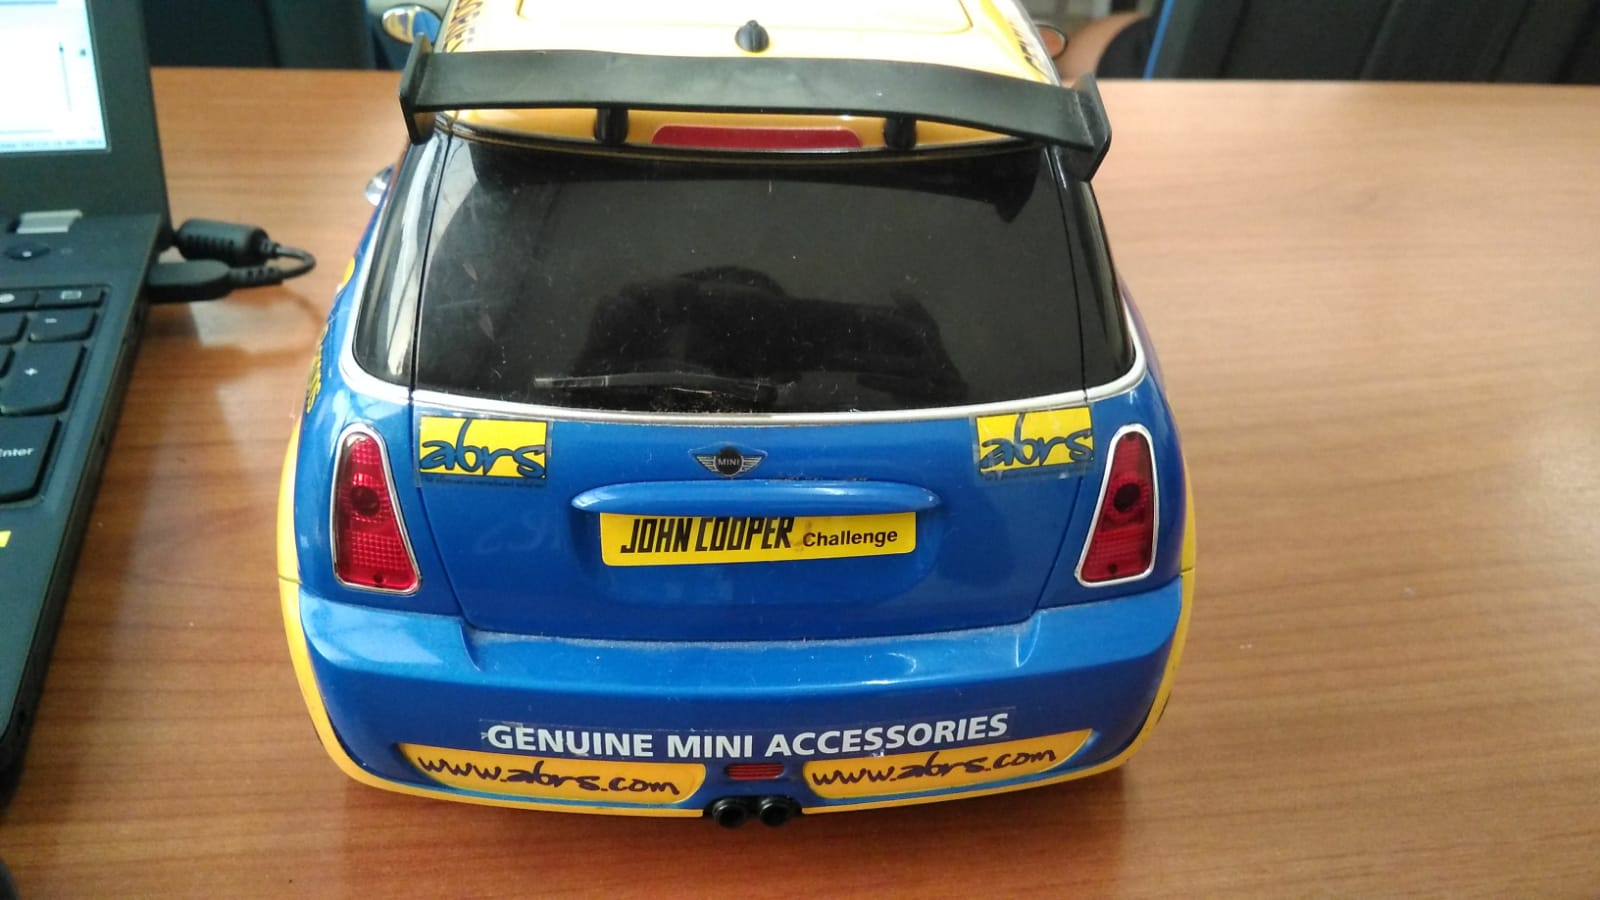
\includegraphics[width=\textwidth]{imagenes/robot/vehiculo_trasera.jpeg}
        \caption{Vista trasera}
        \label{fig:mouse}
    \end{subfigure}
    \caption{Vehículo SensorRS \protect\footnotemark.}\label{fig:animals}
\end{figure}


\footnotetext{Vehículo desarrollado con la finalidad de integrarlo en la aplicación RobotUI. Su desarrollo y características quedan descritas en el capítulo \ref{chap:robot_construccion}.}


\section{Objetivos}
\label{sec:objetivos}

Como hemos visto, se requiere de multitud de conocimientos a la hora de afrontar un proyecto robótico con ciertas garantías. Este proyecto trata de la elaboración 
de un vehículo robótico de fácil construcción mediante la utilización de componentes fácilmente adquiribles y de reducido coste.\\

Dicho robot irá destinado al área de la exploración, buscando, al menos, reducir la exposición de personas a zonas peligrosas ayudando a las labores de rastreo 
o incursión en lugares en principio inalcanzables o de dificultoso acceso.\\

En la presente memoria se abarcará la descripción del diseño, construcción y control de un Robot autómata teledirigido a base de una placa Arduino y Raspberry Pi dotado de multitud de sensores que ayuden a proporcionar 
información del entorno más próximo en el que se encuentra.\\

En lo referente al área de la programación, más concretamente con la programación de microcontroladores\footnote{Un microcontrolador (abreviado μC, UC o MCU) es un circuito integrado programable, capaz de 
ejecutar las órdenes grabadas en su memoria. Está compuesto de varios bloques funcionales, los cuales cumplen una tarea específica. Un microcontrolador incluye en su interior las
tres principales unidades funcionales de una computadora: unidad central de procesamiento, memoria y periféricos de entrada/salida. } permitirá crear un sistema fácilmente escalable
donde agregar nuevos sensores no suponga un elevado esferzo.\\

En definitiva, este proyecto intenta demostrar que sin la necesiad de grandes conocimientos en programación, junto con pequeñas nociones de electrónica básica, que cualquier
persona pueda elaborar un proyecto robótico de similares características. Evitanto que multitud de personas vean el no disponer de grandes conocimientos en la materia sean un impedimento a la 
hora de comenzar a desarrollar sus ideas.\\


\section{Acerca de este documento}

El documento se ha sido elaborado en un lenguaje claro y sencillo para permitir que un estudiante universitario de Ingeniería Informática pueda comprender los contenidos sin apenas dificultad añadida.\\

Este documento se organiza en los siguientes capítulos:\\

\begin{itemize}

\item En el capítulo \ref{chap:introducción}, Introducción, se comentan las razones que han motivado la creación de este proyecto, así como el propósito del mismo.

\item En el capítulo \ref{chap:conceptos-básicos}, Conceptos básicos, se incluyen definiciones de aquellos conceptos considerados de interés para la correcta comprensión del contenido de la presente memoria.

\item En el capítulo \ref{chap:herramientas}, Estado del arte y herramientas utilizadas, se realiza una descripción de las diferentes elementos hardware y software empleados durante el desarrollo del proyecto y necesarios para la utilización del mismo. Así como una breve descripción del conocimiento acumulado y tecnologías existentes hasta la fecha.

\item En el capítulo \ref{chap:requisitos}, Análisis de requisitos, se realiza un análisis sobre la metodología empleada para el desarrollo del proyecto, describiendo
los modelos de ciclo de vida utilizados en el caso del desarrollo software y la descripción de los requisitos funcionales y no funcionales del mismo.

\item En el capítulo \ref{chap:montaje}, Construcción del robot, se recogen aquellos aspectos referentes al montaje del robot SensorRS, conexionado y sensores utilizados. 

\item En el capítulo \ref{chap:desarrollo-software}, Desarrollo software, se recogen aquellos aspectos referentes a la programación del robot y los diferentes canales de comunicación existentes.

\item En el capítulo \ref{chap:pruebas}, Pruebas, se detallan las pruebas a las que se ha sometido el sistema.

\item En el capítulo \ref{chap:planificación}, Organización temporal, se recoge todo lo que concierne a la distribución y duración de cada una de las tareas llevadas a cabo durante el desarrollo del proyecto que el presente documento describe.

\item En el capítulo \ref{chap:manual-usuario}, Guía de usuario, se describen los diferentes aspectos necesarios para la correcta utilización del conjunto software y hardware de los que se compone el presente proyecto.

\item En el capítulo \ref{chap:conclusiones}, Comentarios finales, se hace mención de las conclusiones obtenidas tras la realización del proyecto además de las posibles mejoras aplicables y presupuesto.

\item En el apéndice Anexos  \hyperref[appendix:anexos]{A}, aparecen los manuales de instalación del software que ha sido necesario para la realización del proyecto.

\end{itemize}
